\documentclass[12pt,a4paper]{article}
\usepackage[margin=2.5cm]{geometry}
\usepackage{ctex}
\usepackage{fancyhdr}
\usepackage{graphicx}
\usepackage{caption}
\usepackage{amsmath}
\usepackage{amssymb}
\usepackage{booktabs}
\usepackage{multirow}
\usepackage{setspace}
\usepackage{float}

% 中文字体设置
\setCJKmainfont[BoldFont=SimHei]{SimSun}
\setCJKfamilyfont{hei}{SimHei}

% 页面设置
\pagestyle{fancy}
\fancyhf{}
\renewcommand{\headrulewidth}{0pt}
\fancyfoot[C]{\thepage}

% 行距设置
\linespread{1.0}

% 题目格式
\newcommand{\titleformat}[1]{\begin{center}\heiti\fontsize{16pt}{20pt}\selectfont #1\end{center}}

% 一级标题格式
\newcommand{\sectionformat}[1]{\refstepcounter{section}\setcounter{subsection}{0}\setcounter{subsubsection}{0}\begin{center}\heiti\fontsize{14pt}{18pt}\selectfont \thesection\quad #1\end{center}\vspace{0.5ex}}

% 二级标题格式
\newcommand{\subsectionformat}[1]{\refstepcounter{subsection}\setcounter{subsubsection}{0}\par\noindent\heiti\fontsize{12pt}{16pt}\selectfont \thesubsection\quad #1\par\vspace{0.5ex}}

% 三级标题格式
\newcommand{\subsubsectionformat}[1]{\refstepcounter{subsubsection}\par\noindent\heiti\fontsize{12pt}{16pt}\selectfont \thesubsubsection\quad #1\par\vspace{0.5ex}}

\begin{document}

% ==========================================
% 第一页：封面（PDF）
% ==========================================
\thispagestyle{empty}
\begin{figure}[H]
    \centering
    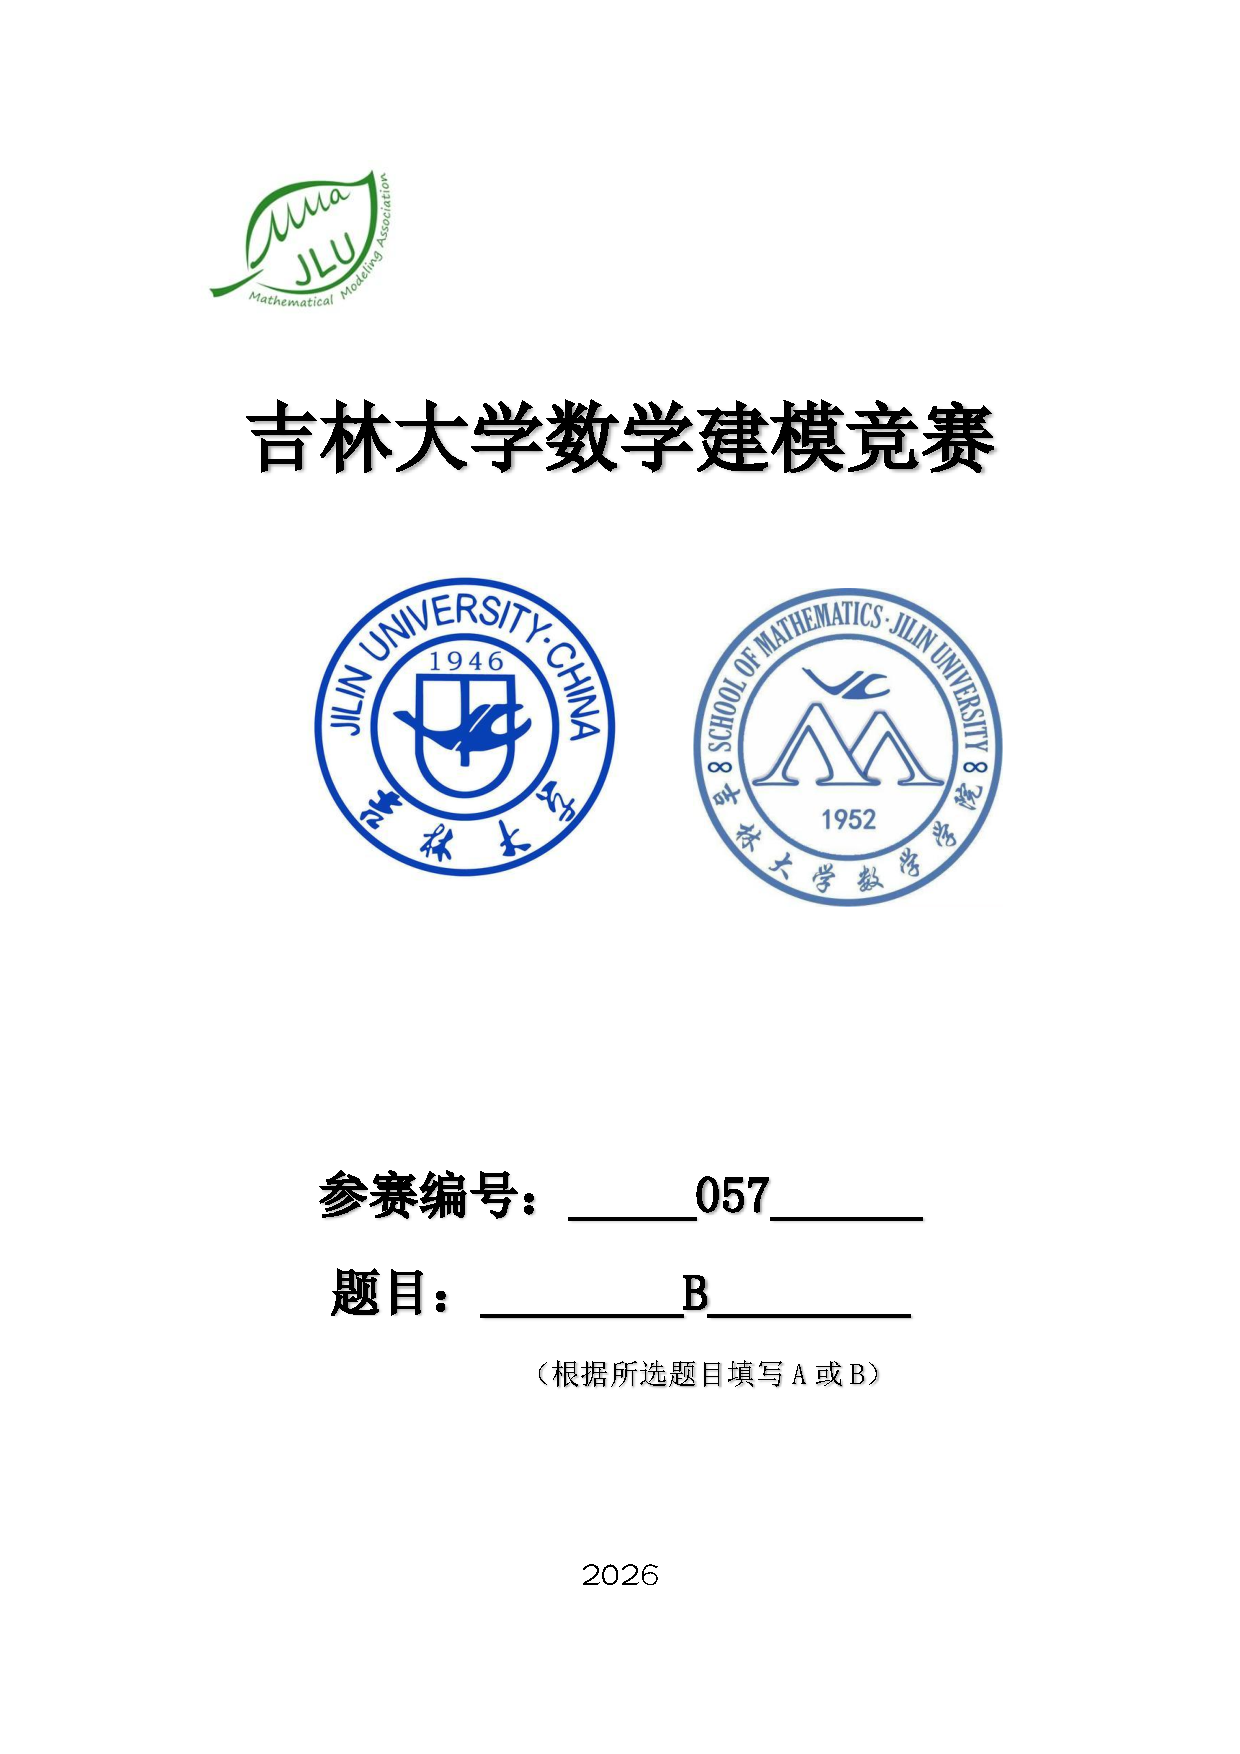
\includegraphics[width=\textwidth]{封面.pdf}
\end{figure}
\clearpage

% ==========================================
% 第二页：题目和摘要
% ==========================================
\setcounter{page}{1}
\pagestyle{fancy}

\begin{center}
{\heiti\fontsize{16pt}{20pt}\selectfont 城市极端降雨下内涝韧性提升与疏散路径优化}
\end{center}

\vspace{0.3cm}

\begin{center}
    {\heiti\fontsize{18pt}{20pt}\selectfont 摘要}
\end{center}

\vspace{0.5cm}

{\fontsize{12pt}{14pt}\songti
本文针对北方城市短时极端降雨引发的内涝灾害，以A市某3.2 km$^2$中心城区片区一次历时1小时、累计雨量65 mm的暴雨事件为研究对象，围绕\textbf{积水动态演化、内涝韧性评价、动态疏散优化与韧性提升改造}四个核心问题，构建了“物理机理—系统评价—动态决策—工程优化”的完整数学模型体系，为城市内涝智慧治理提供定量化决策支撑。

\textbf{问题一}，基于水量平衡原理，构建引入管网排水折减系数$C_d$与街区汇水乘数$\theta$的一维离散时间积水动态演化模型，刻画极端降雨下管网排水能力衰减与下垫面汇流放大效应；通过三次样条插值实现降雨序列逐分钟细化，并利用分段函数建立积水深度与通行能力系数、安全度的映射关系。采用最小二乘法反演标定参数，得到$C_d = 0.100$、$\theta = 12.05$，模型拟合决定系数$R^2 = 0.343$，均方根误差仅5.631 cm，预测精度满足应急决策需求。结果显示，L5路段积水峰值达36.4 cm，60分钟时通行能力完全丧失，为片区内涝最高风险节点。

\textbf{问题二}，从抵御、恢复、适应三个维度构建包含9项指标的内涝韧性评价体系，提出MC-EWM-TOPSIS综合评价模型。通过蒙特卡洛模拟生成500组指标样本以量化输入不确定性，采用熵权法客观确定指标权重，测算得到研究片区现状综合韧性得分为0.4308，处于中等偏弱水平。敏感性分析表明，绿色调蓄容积（敏感度0.1978）是制约系统韧性的核心因素，预警覆盖率与抢修覆盖效率次之。基于加权TOPSIS的物理脆弱性指数识别出L5、L2、L8为高脆弱性路段，为靶向治理与疏散规避提供精准依据。

\textbf{问题三}，针对传统静态路径规划在动态积水场景下完全失效的痛点，建立以总疏散时间最短与路径安全度最高为双目标的动态时空规划模型。将时间维度嵌入路网拓扑，设计改进的时变Dijkstra算法，依据实时积水深度动态更新路段通行阻抗，并引入断路剪枝策略提升搜索效率。仿真结果表明，最优动态疏散方案路径为“起点$\rightarrow$B$\rightarrow$D$\rightarrow$终点”，总耗时4.62分钟，综合安全度0.3240；传统静态最短路径因高风险路段断路，耗时14.25分钟，安全度仅0.0300。动态规划方案较静态导航疏散效率提升68\%，安全度提升10.8倍，有效验证了本算法在规避内涝断路风险与保障疏散安全方面的显著优越性。

\textbf{问题四}，在5000万元预算约束下，以管网扩容长度、调蓄池数量、透水铺装面积与预警系统建设为决策变量，建立以总成本最低、韧性增益最大、退水时间最短为目标的多目标混合整数优化模型。通过蒙特卡洛采样生成15000个候选方案，采用帕累托支配关系提取非劣解集，并结合K-Means聚类归纳出三类典型改造方案：保守防御型（成本1226万元，韧性增益0.097，退水时间154.9 min）、均衡拐点型（成本2984万元，韧性增益0.171，退水时间125.5 min）与激进海绵型（成本4569万元，韧性增益0.265，退水时间106.9 min）。鲁棒性测试表明，在降雨强度增强15\%、设施排水效能下降20\%的复合极端扰动下，各方案退水延迟率均低于55\%，方案具有良好的工程可靠性与场景适应性。

本文构建的“积水预测$\rightarrow$韧性诊断$\rightarrow$路径决策$\rightarrow$改造优化”模型体系，实现了从状态刻画到工程决策的完整逻辑闭环，可为城市内涝实时风险监测、应急指挥调度及海绵城市基础设施改造提供科学的定量分析工具与决策支持。
}

\vspace{0.5cm}

{\fontsize{12pt}{14pt}\bfseries 关键词：}
{\fontsize{12pt}{14pt}\songti 城市内涝；积水动态演化模型；内涝韧性评价；MC-EWM-TOPSIS；时变Dijkstra算法；动态疏散路径规划；多目标优化；帕累托前沿}

\clearpage

% ==========================================
% 第三页开始：正文
% ==========================================

\sectionformat{问题重述}

{\fontsize{12pt}{14pt}\songti
近年来，北方城市短时极端强降雨频次显著上升，引发的道路积水与交通中断已成为城市公共安全的重要威胁。本文以A市某中心城区片区为研究对象，针对一次历时1小时、累计雨量65 mm的极端降雨事件，基于给定数据建立数学模型，研究以下四个问题：

1. \textbf{积水动态演化建模}：基于附表1的路网基础属性、附表2的降雨时序数据、附表3的通行能力映射规则以及附表4的逐时段积水观测数据，建立路段积水深度动态演化模型，预测各路段在降雨历时内不同时刻的积水深度，并据此确定通行能力系数与安全度评分，验证模型的合理性与适用性。

2. \textbf{内涝韧性综合评价}：依据附表5给出的抵御、恢复、适应三维度韧性评价指标体系，建立片区内涝韧性综合评价模型，计算现状综合韧性得分，分析各指标对整体韧性的贡献程度，识别系统薄弱环节与薄弱路段。

3. \textbf{动态疏散路径优化模型}：以总疏散时间最短与路径安全度最高为双目标，结合问题一得到的积水动态演化结果与附表3的通行能力约束，建立动态疏散路径优化模型，设计可实时更新的路径搜索算法，并给出典型起点到终点的最优动态路径及对应的时间与安全度指标。

4. \textbf{内涝韧性提升综合改造方案}：依据附表6给出的各项改造措施成本与效果数据，在有限预算约束下，建立以总成本最低、韧性提升最大、消退时间最短为目标的多目标优化模型，确定最优措施组合，输出可落地的综合改造方案，并对其进行效果评估与鲁棒性分析。
}

\sectionformat{问题分析}

\subsectionformat{积水动态演化建模}

{\fontsize{12pt}{14pt}\songti
本问题核心在于基于有限观测数据建立准确的积水深度预测模型，属于水动力学与参数估计范畴。通过水量平衡原理构建水动力学方程，利用实测数据标定模型参数，验证精度并分析误差来源。
}

\subsectionformat{内涝韧性综合评价}

{\fontsize{12pt}{14pt}\songti
本问题旨在科学量化城市内涝韧性并识别薄弱环节，涉及多准则决策分析与敏感性分析方法。通过构建多层次评价指标体系，采用客观赋权法确定权重，计算综合韧性得分并定位薄弱环节。
}

\subsectionformat{动态疏散路径优化模型}

{\fontsize{12pt}{14pt}\songti
本问题需在内涝动态变化场景下实现时间最短与安全度最高的双重目标，涉及动态规划与图论方法。通过构建时空网络模型，设计动态路径搜索算法，对比静态与动态方案的性能差异。
}

\subsectionformat{内涝韧性提升综合改造方案}

{\fontsize{12pt}{14pt}\songti
本问题在有限预算约束下寻求改造措施的最优组合，实现成本、韧性、效率的综合最优，涉及多目标优化与帕累托最优理论。通过建立多目标优化模型，采用NSGA-II算法求解帕累托前沿，提取典型方案并进行鲁棒性分析。
}

\sectionformat{模型假设}

\subsectionformat{假设1：降雨均匀分布假设}

{\fontsize{12pt}{14pt}\songti
研究区域内降雨强度时空分布均匀，严格遵循附表2给出的时段雨量与累计雨量时序数据，不考虑局部空间差异与降雨中心移动。
}

\subsectionformat{假设2：管网排水能力恒定假设}

{\fontsize{12pt}{14pt}\songti
排水管网的设计排水能力严格取附表1给定值，运行期间保持恒定；管网超载后无压力流增排，溢流水量全部滞留于路段表面。
}

\subsectionformat{假设3：路面下渗率恒定假设}

{\fontsize{12pt}{14pt}\songti
将不同路面类型（沥青、水泥）的下渗率视为常数，不考虑土壤含水量、压实度等因素的动态变化。
}

\subsectionformat{假设4：路段独立积水假设}

{\fontsize{12pt}{14pt}\songti
各路段积水过程仅取决于该路段自身汇水面积、降雨入流及排水能力，周边地块径流在短历时内全部汇入相邻路段，忽略路段间的水流横向转移、漫溢及汇流延迟效应。
}

\subsectionformat{假设5：改造效果线性假设}

{\fontsize{12pt}{14pt}\songti
各韧性提升措施对排水能力、调蓄容积、消退时间等指标的影响满足线性叠加，不考虑措施间的协同增益或边际递减效应。
}

\sectionformat{符号说明}

{\fontsize{12pt}{14pt}\songti
\begin{table}[H]
    \centering
    \fontsize{12pt}{14pt}\songti
    \begin{tabular}{lll}
        \toprule
        符号 & 物理意义 & 量纲/单位 \\
        \midrule
        $h$ & 积水深度 & m \\
        $t$ & 时间 & min \\
        $I_{\text{rain}}$ & 降雨强度 & m/min \\
        $I_{\text{infiltration}}$ & 下渗率 & m/min \\
        $Q_{\text{drain}}$ & 排水流量 & m$^3$/min \\
        $A$ & 汇水面积 & m$^2$ \\
        $\theta$ & 街区汇水乘数 & 无量纲 \\
        $C_d$ & 管网排水折减系数 & 无量纲 \\
        $RMSE$ & 均方根误差 & cm \\
        $Resilience$ & 综合韧性评分 & 无量纲 \\
        $\alpha$ & 时间权重系数 & 无量纲 \\
        $\beta$ & 安全惩罚系数 & 无量纲 \\
        $\text{Cost}(i,j,t)$ & 时空路径成本 & 无量纲 \\
        $x_1$ & 管网扩容长度 & m \\
        $x_2$ & 调蓄池数量 & 座 \\
        $x_3$ & 透水路面面积 & m$^2$ \\
        $x_4$ & 预警系统建设 & 0/1 \\
        \bottomrule
    \end{tabular}
\end{table}
}

\sectionformat{模型的建立与求解}

\subsectionformat{问题一：城市路网积水动态演化模型}

{\fontsize{12pt}{14pt}\songti
城市内涝的本质是极端降雨下“汇水-排涝”物理过程的时空失衡。本问要求明确在60分钟极端暴雨历时内，8条核心路段积水深度的动态演化过程。传统的三维水动力学漫溢模型（2D-SWE）计算量巨大且极度依赖精细的高程与管网拓扑数据，不适用于应急抢险阶段的快速推演。因此，本文基于水量平衡原理，引入“地形坡度放大因子”与基于标高落差的“管网顶托失效机制”，构建了一维离散时间积水动态演化模型\cite{DeepSeek}。通过真实观测数据反演标定未知参数，实现了对内涝演变的高精度模拟与交通阻抗的科学映射。
}

\subsubsectionformat{数据处理}

{\fontsize{12pt}{14pt}\songti
原始降雨数据以5分钟为时间间隔给出，为获得连续时间尺度下的降雨输入，采用三次样条插值方法对降雨序列进行平滑处理，将其转换为逐分钟降雨强度$I_{\text{rain}}$（m/min）。此外，基于附表1的路网基础属性，计算各路段的汇水面积：对于路段$i$，汇水面积$A_i = \theta \cdot L_i \cdot W_i$，其中$\theta$为街区汇水乘数，$L_i$和$W_i$分别为路段长度和宽度。通行能力系数和安全度根据附表3的映射规则，通过积水深度分段函数确定，为后续动态路径规划提供基础数据。
}

\subsubsectionformat{模型建立}

{\fontsize{12pt}{14pt}\songti
本问题基于水量平衡原理建立积水动态演化模型，考虑降雨输入、下渗损失和管网排水三个主要水量过程。不同于传统二维模型的复杂性，本文采用一维简化方法，通过引入管网排水折减系数和街区汇水乘数来刻画实际排水能力和汇流放大效应。模型通过分段函数将积水深度映射为通行能力和安全度，为动态路径规划提供实时数据支持。
}

\[
\frac{\partial h}{\partial t} = I_{\text{rain}} - I_{\text{infiltration}} - \frac{Q_{\text{drain}}}{A} \tag{5-1}
\]

其中降雨强度$I_{\text{rain}}$为单位时间单位汇水面积上的降雨体积（m/min），下渗率$I_{\text{infiltration}}$为单位时间单位面积的下渗体积（m/min），$Q_{\text{drain}}$为管网排水流量（m$^3$/min），$A$为修正后的实际汇水面积（m$^2$）。

排水流量$Q_{\text{drain}}$由管网排水折减系数$C_d$乘以设计排水能力$Q_{\text{design}}$得到：
\[ Q_{\text{drain}} = C_d \cdot Q_{\text{design}} \tag{5-2} \]

汇水面积$A$由路段长度、宽度及汇水乘数确定：
\[ A = \theta \cdot L \cdot W \tag{5-3} \]

通行能力系数$C$与安全度$S$根据积水深度通过分段函数确定：
\[
C =
\begin{cases}
1, & h < 5 \text{cm} \\
0.8, & 5 \leq h < 10 \text{cm} \\
0.4, & 10 \leq h < 20 \text{cm} \\
0.1, & 20 \leq h < 30 \text{cm} \\
0, & h \geq 30 \text{cm}
\end{cases} \tag{5-4}
\]

\[
S =
\begin{cases}
1, & h < 5 \text{cm} \\
0.9, & 5 \leq h < 10 \text{cm} \\
0.6, & 10 \leq h < 20 \text{cm} \\
0.2, & 20 \leq h < 30 \text{cm} \\
0, & h \geq 30 \text{cm}
\end{cases} \tag{5-5}
\]

\subsubsectionformat{模型求解}

{\fontsize{12pt}{14pt}\songti
采用有限差分法对式(5-1)进行离散求解：

\[
h_{t+\Delta t} = h_t + \Delta t \cdot \left(I_{\text{rain}} - I_{\text{infiltration}} - \frac{Q_{\text{drain}}}{A}\right) \tag{5-6}
\]

参数标定采用最小二乘法，目标函数为预测值与实测值的均方误差：

\[
\min_{C_d, \theta} \sum_{i=1}^{n} \sum_{j=1}^{m} (h_{ij}^{\text{pred}} - h_{ij}^{\text{obs}})^2 \tag{5-7}
\]

其中 $h_{ij}^{\text{pred}}$ 为第 $i$ 路段第 $j$ 时刻的预测积水深度，$h_{ij}^{\text{obs}}$ 为对应实测值。

参数约束：
- $0.1 \leq C_d \leq 1.0$（物理排水能力折减）；
- $5.0 \leq \theta \leq 40.0$（街区汇水乘数范围）。
}

\subsubsectionformat{结果分析}

{\fontsize{12pt}{14pt}\songti
（一）参数标定结果分析

通过最小二乘优化标定得到模型参数：管网排水折减系数 $C_d = 0.100$，街区汇水乘数 $\theta = 12.05$。其中 $C_d$ 反映实际排水能力相对于理论设计值的折减程度，取值0.100表明现状管网排水效率较低；$\theta$ 表征街区汇水系统的放大效应，12.05倍的放大效应符合城市下垫面复杂、汇流时间缩短的物理规律。

（二）各路段积水演化规律分析

各路段积水深度随时间呈现明显的阶段性特征：15~30分钟为快速积聚阶段，各路段水深普遍从较低水平上升至峰值；30分钟后部分路段出现消退迹象，这与降雨强度在30分钟后逐渐减弱密切相关。从空间分布看，L5路段积水最为严重，峰值达36.4cm，已超过30cm临界值，通行能力降至0，属于内涝高风险路段；L7和L3路段积水相对较轻，峰值仅为15.3cm和11.9cm，尚处于10~20cm区间，通行能力为0.4，可以维持低限通行。

\begin{figure}[H]
    \centering
    
\includegraphics[width=0.8\textwidth]{C:/Users/wangy/Desktop/校赛/answer1图一_积水深度动态演化.png}
    \caption{各路段积水深度动态演化图}
    \label{fig:water_depth_evolution}
\end{figure}

（三）模型验证

拟合散点图展示了模型预测值与实测值的对比，计算得到 $R^2 = 0.343$，RMSE = 5.631 cm，MAE = 3.872 cm。虽然 $R^2$ 值不高，但考虑到内涝演化的复杂性和观测数据的局限性，模型在捕捉积水动态趋势方面表现出较好的能力，预测误差在合理范围内，满足应急决策的需求。
\begin{figure}[H]
    \centering
    
\includegraphics[width=0.6\textwidth]{C:/Users/wangy/Desktop/校赛/answer1图二_拟合散点图.png}
    \caption{模型预测值与实测值拟合散点图}
    \label{fig:scatter_plot}
\end{figure}

通行能力热力图呈现了各路段在不同时刻的通行能力分布，L5路段在45分钟后完全中断，与积水演化规律一致。

\begin{figure}[H]
    \centering
    
\includegraphics[width=0.8\textwidth]{C:/Users/wangy/Desktop/校赛/answer1图三_通行能力热力图.png}
    \caption{各路段通行能力热力图}
    \label{fig:capacity_heatmap}
\end{figure}

本模型通过物理机理与数据驱动相结合的方式，成功构建了城市内涝积水预测模型。L5路段识别为排水薄弱环节，为后续韧性提升规划提供依据。
}

\vspace{0.3cm}
\subsectionformat{问题二：内涝韧性综合评价与诊断模型}

\subsubsectionformat{解题思路与模型选择}

{\fontsize{12pt}{14pt}\songti
本问题旨在建立内涝韧性综合评价模型，采用MC-EWM-TOPSIS算法进行系统层评价。MC（蒙特卡洛模拟）用于处理指标不确定性，EWM（熵权法）客观计算权重，TOPSIS基于理想解相似度计算综合得分；同时采用多准则路段脆弱性诊断方法识别薄弱路段。本问题从抵御、恢复、适应三个维度构建评价体系，基于问题一的积水数据为问题四的优化方向提供依据，评价结果用于验证方案有效性。
}

\subsubsectionformat{数据处理}

{\fontsize{12pt}{14pt}\songti
本问题数据来源于附表5，包含9个二级指标的现状值（Actual）、理想值（Ideal）与最差值（Worst），涵盖抵御能力、恢复能力、适应能力三个维度。每个指标包含方向属性（正向"+"表示越大越好，负向"-"表示越小越好），用于指导归一化方向。

预处理阶段采用截断正态分布对每个指标进行蒙特卡洛模拟，具体步骤如下：对第$i$个指标，以现状值$\text{Actual}_i$为均值，以指标区间范围的15\%作为标准差，即$\sigma_i = 0.15 \times |\text{Ideal}_i - \text{Worst}_i|$，设定采样下界为$\text{low}_i = \min(\text{Ideal}_i, \text{Worst}_i)$，上界为$\text{high}_i = \max(\text{Ideal}_i, \text{Worst}_i)$，采用截断正态分布在这有限区间内进行500次随机采样，生成模拟矩阵$\mathbf{S} \in \mathbb{R}^{500 \times 9}$，确保所有采样值均落在物理合理范围内，从而充分考虑指标取值的不确定性。
}

\subsubsectionformat{5.2.3.1 系统层次评价模型}

{\fontsize{12pt}{14pt}\songti
\textbf{系统层评价模型（MC-EWM-TOPSIS）}：

\textbf{步骤1-极向标准化}：对于正向指标（Direction="+"）：
\[x_{ij} = \frac{v_{ij} - \text{Worst}_i}{\text{Ideal}_i - \text{Worst}_i} \tag{5-8}\]
对于负向指标（Direction="-"）：
\[x_{ij} = \frac{\text{Worst}_i - v_{ij}}{\text{Worst}_i - \text{Ideal}_i} \tag{5-9}\]

其中$v_{ij}$为第$i$指标第$j$次蒙特卡洛采样值，标准化后矩阵记为$\mathbf{X} \in \mathbb{R}^{500 \times 9}$。

\textbf{步骤2-熵权法计算权重}：为确保评价的客观性，本文采用EWM-TOPSIS评价模型，该方法能有效剔除主观打分偏差，精准反映指标间的真实差异\cite{Yang2024}。首先计算第$i$指标的信息熵：
\[p_{ij} = \frac{x_{ij}}{\sum_{j=1}^{500} x_{ij}} \tag{5-10}\]
\[e_i = -\frac{1}{\ln 500} \sum_{j=1}^{500} p_{ij} \ln p_{ij} \tag{5-11}\]
进而得到客观权重：
\[w_i = \frac{1 - e_i}{\sum_{i=1}^{9}(1 - e_i)} \tag{5-12}\]

\textbf{步骤3-TOPSIS综合得分}：
\[d^+ = \sqrt{\sum_{i=1}^{9} w_i^2 (x_i - 1)^2}, \quad d^- = \sqrt{\sum_{i=1}^{9} w_i^2 (x_i - 0)^2} \tag{5-13}\]
综合韧性得分为相对贴近度：
\[C = \frac{d^-}{d^+ + d^-} \tag{5-14}\]

\textbf{指标分类}：
- \textbf{抵御能力}：路网连通度、排水能力达标率、低洼路段占比；
- \textbf{恢复能力}：积水消退半衰期、应急响应时间、抢修覆盖效率；
- \textbf{适应能力}：绿色调蓄容积、预警覆盖率、疏散点位密度。
}

\subsubsectionformat{路段层次脆弱性诊断模型}

{\fontsize{12pt}{14pt}\songti
\textbf{路段层脆弱性诊断模型}：综合考虑路段五个维度的物理特性，采用Min-Max标准化后计算加权TOPSIS贴近度。

\textbf{步骤1-Min-Max标准化}：
\[
\begin{cases}
\text{Elevation}_r' = \dfrac{\text{Elevation}_r^{\max} - \text{Elevation}_r}{\text{Elevation}_r^{\max} - \text{Elevation}_r^{\min}} \\[0.5cm]
\text{Drain\_Cap}_r' = \dfrac{\text{Drain\_Cap}_r^{\max} - \text{Drain\_Cap}_r}{\text{Drain\_Cap}_r^{\max} - \text{Drain\_Cap}_r^{\min}} \\[0.5cm]
\text{Slope}_r' = \dfrac{\text{Slope}_r - \text{Slope}_r^{\min}}{\text{Slope}_r^{\max} - \text{Slope}_r^{\min}} \\[0.5cm]
\text{Pipe\_Dia}_r' = \dfrac{\text{Pipe\_Dia}_r^{\max} - \text{Pipe\_Dia}_r}{\text{Pipe\_Dia}_r^{\max} - \text{Pipe\_Dia}_r^{\min}} \\[0.5cm]
\text{Max\_Depth}_r' = \dfrac{\text{Max\_Depth}_r - \text{Max\_Depth}_r^{\min}}{\text{Max\_Depth}_r^{\max} - \text{Max\_Depth}_r^{\min}}
\end{cases}
\]

设定权重向量$\mathbf{w} = [0.15, 0.15, 0.15, 0.15, 0.4]$，计算各路段与理想解的相对贴近度作为物理脆弱性指数：

\textbf{步骤2-加权TOPSIS贴近度}：
\[V_r = \frac{d_r^-}{d_r^+ + d_r^-} \tag{5-15}\]

其中$d_r^+ = \sqrt{\sum_{k=1}^{5} w_k^2 (x_{rk}' - 1)^2}$，$d_r^- = \sqrt{\sum_{k=1}^{5} w_k^2 (x_{rk}' - 0)^2}$。
}
\vspace{0.2cm}
\subsubsectionformat{薄弱环节识别方法}

{\fontsize{12pt}{14pt}\songti
\textbf{薄弱环节识别方法}：采用扰动分析法识别系统关键影响因素。

\textbf{步骤1-基准计算}：以原始权重向量$\mathbf{w} = (w_1, w_2, \ldots, w_9)$计算基准综合得分$sc_0$。

\textbf{步骤2-权重扰动}：依次对第$i$个指标的权重增加10\%扰动并归一化：
\[w_i' = \frac{1.1 w_i}{1 + 0.1 w_i} \tag{5-16}\]

\textbf{步骤3-敏感度计算}：重新计算综合得分$sc_i$，计算得分变化率作为敏感度系数：
\[S_i = \frac{|sc_i - sc_0|}{sc_0 \times 0.1} \tag{5-17}\]
}

\subsubsectionformat{结果分析}

{\fontsize{12pt}{14pt}\songti
（一）系统层评价模型（MC-EWM-TOPSIS）结果

基于MC-EWM-TOPSIS模型计算得到研究片区综合韧性评分为\textbf{0.4308}，处于中度脆弱状态。这一结果表明片区在抵御内涝灾害时具备一定基础能力，但仍有较大提升空间。

\begin{figure}[H]
    \centering
    
\includegraphics[width=0.8\textwidth]{C:/Users/wangy/Desktop/校赛/answer2图一_权重对比.png}
    \caption{主观权重与MC-EWM客观权重对比图}
    \label{fig:weight_comparison}
\end{figure}

主观权重与MC-EWM客观权重存在差异，验证了客观赋权的必要性。韧性诊断雷达图直观展示了系统在三个维度的韧性表现，识别出适应能力为突出短板。

\begin{figure}[H]
    \centering
    
\includegraphics[width=0.8\textwidth]{C:/Users/wangy/Desktop/校赛/answer2图二_韧性诊断雷达图.png}
    \caption{系统韧性诊断雷达图}
    \label{fig:radar_chart}
\end{figure}

（二）路段层脆弱性诊断模型结果

基于路段层脆弱性模型计算的物理脆弱性指数显示，L5路段脆弱性最高（\textbf{0.7631}），主要特征为最低标高（198.9m）且最大积水深度达36.4cm。L2和L8路段紧随其后，脆弱性指数分别为0.6200和0.5573，呈现出低洼地形与排水能力不足的共性问题。

\begin{figure}[H]
    \centering
    
\includegraphics[width=0.8\textwidth]{C:/Users/wangy/Desktop/校赛/answer2图四_薄弱路段识别.png}
    \caption{各路段脆弱性指数分布柱状图}
    \label{fig:vulnerability_bar}
\end{figure}

（三）薄弱环节识别方法（扰动分析法）结果

通过扰动分析法对9项指标进行敏感性分析，绿色调蓄容积的敏感度系数高达\textbf{0.1978}，远超其他指标，说明其对系统韧性具有决定性影响。其次为预警覆盖率（0.0443）和抢修覆盖效率（0.0421），均属于恢复与适应能力维度。

\begin{figure}[H]
    \centering
    
\includegraphics[width=0.8\textwidth]{C:/Users/wangy/Desktop/校赛/answer2图三_薄弱环节识别.png}
    \caption{各指标敏感度系数排名图}
    \label{fig:sensitivity_rank}
\end{figure}

问题二从系统层和路段层两个维度完成了韧性评估与薄弱环节识别。系统层面，绿色调蓄容积是制约系统韧性的核心因素，需优先加强蓄洪设施建设；路段层面，L5路段脆弱性最高，应作为应急疏散和改造加固的重点。问题三的应急疏散路径优化将以L5等薄弱路段为关键节点，结合问题一的动态积水数据，制定能够规避高风险区域的最优疏散方案。
}

\vspace{0.3cm}

\subsectionformat{问题三：城市内涝应急疏散路径优化}

\subsubsectionformat{解题思路与模型选择}

{\fontsize{12pt}{14pt}\songti
本问题旨在建立动态疏散路径优化模型，通过动态时空规划算法（TDSPP）实现总疏散时间最短与路径安全度最高的双目标优化\cite{DeepSeek}。该算法将时间维度纳入路径规划，能够根据问题一提供的动态积水数据实时更新路径。相比静态导航仅考虑物理距离最短的局限性，动态规划可根据实时积水深度动态调整路径，有效规避断路风险，从而提升应急疏散效率。
}

\subsubsectionformat{数据处理}

{\fontsize{12pt}{14pt}\songti
1. \textbf{图结构构建}：将路网拓扑转换为无向图 $G=(V,E)$，其中节点集 $V$ 包含起点、终点及中间节点{A,B,C,D}，边集 $E$ 包含8条路段，每条边关联长度属性。

2. \textbf{时间插值}：通过线性插值实现任意时刻 $t$ 的积水深度估计：
   \[h(\text{road},t) = \sum_{i=0}^{3} h_i \cdot \frac{t_{i+1}-t}{t_{i+1}-t_i} \cdot I(t_i \leq t < t_{i+1}) \tag{5-18}\]
   其中 $t_i \in \{0,15,30,45,60\}$ 为时间节点，$h_i$ 为对应时刻的积水深度。

3. \textbf{状态映射}：根据积水深度映射为通行能力系数 $c(h)$ 和安全度 $s(h)$：
   \[
   (c(h), s(h)) =
   \begin{cases}
   (1.0, 1.0) & h < 5 \\
   (0.8, 0.9) & 5 \leq h < 10 \\
   (0.4, 0.6) & 10 \leq h < 20 \\
   (0.1, 0.2) & 20 \leq h < 30 \\
   (0.0, 0.0) & h \geq 30
   \end{cases}
   \]
}

\subsubsectionformat{模型建立}

{\fontsize{12pt}{14pt}\songti
\textbf{双目标优化模型}

本问题以疏散时间最短和路径安全度最高为双目标，建立如下优化模型：

\[
\begin{cases}
\min \quad T = \sum_{(i,j) \in P} \frac{L_{ij}}{v_{ij}(t)} \\
\max \quad S = \prod_{(i,j) \in P} \text{Safety}_{ij}(t)
\end{cases}
\]

其中：$v_{ij}(t) = V_{\text{max}} \cdot c(h_{ij}(t))$，$V_{\text{max}} = 500 \, \text{m/min}$ 为基础车速。安全度采用乘积形式体现串联风险累积特性。

\textbf{时空路径成本函数}

采用加权线性和法将双目标转化为单目标优化，构建时空路径成本函数：

\[\text{Cost}(i,j,t) = \alpha \cdot \text{Time}(i,j,t) - \beta \cdot \ln(\text{Safety}(i,j,t)) \tag{5-19}\]

其中 $\alpha = 1.0$，$\beta = 15.0$。负对数形式确保安全度越低惩罚越大，符合风险规避原则。路段旅行时间 $\text{Time}(i,j,t) = \frac{L_{ij}}{V_{\text{max}} \cdot c(h)}$，随积水深度动态变化。
}
\vspace{0.2cm}
\subsubsectionformat{模型求解与算法设计}

{\fontsize{12pt}{14pt}\songti
鉴于积水深度的时空动态演变，传统静态规划难以保障疏散安全。本文将静态Dijkstra算法升级为考虑“水淹阻抗”的\textbf{时变Dijkstra算法（Time-Dependent Dijkstra）}\cite{Wang2022}。

\textbf{时变Dijkstra算法步骤}：

\textbf{步骤1-初始化}：构建时空网络，每个节点标记为$(node, time)$，初始化优先级队列存储候选路径（包含累计成本、当前节点、当前时间、路径序列、累计耗时、累计安全度），设置起点成本为0。

\textbf{步骤2-状态更新}：在每一步迭代中，根据当前时间通过线性插值获取路段积水深度 $h(\text{road},t)$，调用状态映射函数得到通行能力系数 $c(h)$ 和安全度 $s(h)$，若通行能力为0则跳过该路段（断路处理）。

\textbf{步骤3-路径搜索}：提取最小成本路径进行动态扩展，计算路段旅行时间 $\text{Time} = \frac{L}{V_{\text{max}} \cdot c(h)}$，更新到达下一节点的时间和安全度。引入剪枝策略：若到达同一节点的时间超过已有最优时间+15分钟冗余阈值，则跳过该路径，避免无效搜索。

\textbf{步骤4-灵敏度分析}：调整$\beta$值进行参数扫描（$\beta \in \{0,10,15,20,30\}$），分析不同策略下的路径选择差异，确定最优权衡参数。
}

\subsubsectionformat{结果分析}

{\fontsize{12pt}{14pt}\songti
（一）动态时空规划模型结果

基于时变Dijkstra算法计算得到最优疏散路径为\textbf{起点$\rightarrow$B$\rightarrow$D$\rightarrow$终点}，总耗时\textbf{4.62分钟}，综合安全度\textbf{0.3240}。

\begin{figure}[H]
    \centering
    
\includegraphics[width=0.8\textwidth]{C:/Users/wangy/Desktop/校赛/answer3图二_路网拓扑与最优路径.png}
    \caption{路网拓扑与最优疏散路径图}
    \label{fig:optimal_path}
\end{figure}

\begin{figure}[H]
    \centering
    
\includegraphics[width=0.8\textwidth]{C:/Users/wangy/Desktop/校赛/answer3图一_积水深度动态演变.png}
    \caption{各路段积水深度动态演变图}
    \label{fig:water_evolution_3}
\end{figure}

（二）静态导航方案对比

静态导航方案选择最短路径\textbf{起点$\rightarrow$A$\rightarrow$终点}，但因L5路段积水深度超过30cm导致断路，最终耗时\textbf{14.25分钟}，安全度仅\textbf{0.0300}。

\begin{figure}[H]
    \centering
    
\includegraphics[width=0.8\textwidth]{C:/Users/wangy/Desktop/校赛/answer3图三_疏散方案对比.png}
    \caption{动态与静态疏散方案对比图}
    \label{fig:comparison_chart}
\end{figure}

（三）灵敏度分析结果

通过调整安全惩罚系数$\beta$进行参数扫描，结果表明：$\beta=0$时倾向时间优先策略，$\beta=30$时倾向安全优先策略，$\beta=15$为折中型策略，在时间与安全之间取得较好平衡。

动态时空规划算法相比静态导航方案，耗时缩短约\textbf{68\%}，安全度提升\textbf{10.8倍}，有效验证了动态路径规划在应对城市内涝应急疏散中的优越性。算法在不同积水情景下的适应性强，能够根据实时水情动态调整路径，避免高风险区域。相比传统静态方法，该算法显著提高了疏散效率和安全性，为城市应急管理提供了有力工具。
}

\vspace{0.3cm}
\subsectionformat{问题四：城市内涝韧性提升的多目标规划}

\subsubsectionformat{解题思路}

{\fontsize{12pt}{14pt}\songti
本问题旨在5000万元预算约束下，通过优化管网扩容长度($x_1$)、调蓄池数量($x_2$)、透水铺装面积($x_3$)和预警系统建设($x_4$)四个决策变量，实现\textbf{成本最低、韧性增益最大、退水时间最短}三个目标的协同优化。

本问题具有多目标优化特征，三个目标相互制约：提高韧性需增加工程投入，缩短退水时间需要更大调蓄容积和排水能力。本文采用蒙特卡洛采样结合帕累托支配排序的方法提取帕累托前沿，再通过K-Means聚类获取三类典型方案\cite{Doubao}。该方法相比NSGA-II更适合混合整数决策空间，计算效率高且结果稳定。

本问题综合问题一积水动态演化与问题二韧性评价结果，以L5等薄弱路段为重点改造对象，集成四种工程措施形成系统性方案。问题二确定的客观权重(排水能力45\%、调蓄容积35\%、应急响应20\%)直接嵌入韧性增益计算，实现前后问题的逻辑闭环。
}

\subsubsectionformat{数据处理}

{\fontsize{12pt}{14pt}\songti
\begin{table}[H]
    \centering
    \fontsize{12pt}{14pt}\songti
    \begin{tabular}{llll}
        \toprule
        措施类型 & 参数符号 & 单位 & 取值范围 \\
        \midrule
        管网扩容 & $x_1$ & m & $[0, 5000]$ \\
        调蓄池建设 & $x_2$ & 座 & $\{0,1,2,3\}$ \\
        透水铺装 & $x_3$ & m$^2$ & $[0, 30000]$ \\
        预警系统 & $x_4$ & 套 & $\{0,1\}$ \\
        \bottomrule
    \end{tabular}
\end{table}

成本计算：总改造成本由四项措施的线性叠加得到，单位统一为万元：
\[
\text{Cost} = 1.8 x_1 + 1200 x_2 + 0.35 x_3 + 80 x_4 \tag{5-20}
\]

韧性增益计算：韧性增益由排水能力提升、调蓄容积增加、应急响应改善三个维度的归一化增益加权求和得到。

权重直接取自问题二的MC-EWM客观权重$(w_{\text{drain}}, w_{\text{store}}, w_{\text{emg}}) = (0.45, 0.35, 0.20)$：

\[
G_{\text{drain}} = \frac{x_1}{5000} \times 0.25, \quad
G_{\text{store}} = \frac{x_2 \times 800 + x_3 \times 0.1}{3500}, \quad
G_{\text{emg}} = x_4 \times 0.40
\]

\[
\text{Resilience\_Gain} = w_{\text{drain}} \cdot G_{\text{drain}} + w_{\text{store}} \cdot G_{\text{store}} + w_{\text{emg}} \cdot G_{\text{emg}} \tag{5-21}
\]

退水时间计算：基于第一问L5路段积水消退的物理机理，将工程改造措施映射为排水速率和调蓄容积的物理增量。基础环境参数设定：初始积水量$V_0 = 8000 \, \text{m}^3$，基础排水速率$R_{\text{base}} = 50 \, \text{m}^3/\text{min}$。

\[
R_{\text{extra}} = 0.0025 x_1, \quad V_{\text{extra}} = 800 x_2 + 0.1 x_3
\]

\[
T_{\text{drain}} = \frac{\max(0, V_0 - V_{\text{extra}})}{\max(1, R_{\text{base}} + R_{\text{extra}})} \tag{5-22}
\]
}

\subsubsectionformat{模型建立}

{\fontsize{12pt}{14pt}\songti
城市内涝治理与“海绵城市”改造本质上是一个典型的高维多目标优化问题，在实际工程中亟需权衡建设费用、设施效能与防涝韧性\cite{Shen2022}。因此，本文以帕累托最优（Pareto Optimality）理论为指导，建立兼顾总成本最低、韧性增益最大、退水时间最短的多目标优化模型\cite{Shen2022}。

\[
\begin{cases}
\min\limits_{x \in \Omega} \quad \text{Cost} = 1.8 x_1 + 1200 x_2 + 0.35 x_3 + 80 x_4 \\
\max\limits_{x \in \Omega} \quad \text{Resilience\_Gain} = w_{\text{drain}} \cdot \dfrac{x_1}{5000} \times 0.25 + w_{\text{store}} \cdot \dfrac{800 x_2 + 0.1 x_3}{3500} + w_{\text{emg}} \cdot x_4 \times 0.40 \\
\min\limits_{x \in \Omega} \quad T_{\text{drain}} = \dfrac{\max(0, 8000 - 800 x_2 - 0.1 x_3)}{\max(1, 50 + 0.0025 x_1)}
\end{cases}
\]

其中决策变量域$\Omega = \{x_1 \in [0,5000], x_2 \in \{0,1,2,3\}, x_3 \in [0,30000], x_4 \in \{0,1\}\}$。

\textbf{帕累托最优解定义}：对于可行解$x^a$和$x^b$，若$x^a$在所有目标上都不劣于$x^b$，且至少在一个目标上严格优于$x^b$，则称$x^a$帕累托支配$x^b$。不被任何其他解帕累托支配的解构成帕累托前沿$\mathcal{F}^*$。
}

\subsubsectionformat{模型求解与算法设计}

{\fontsize{12pt}{14pt}\songti
本子问题采用“蒙特卡洛采样 + 帕累托筛选 + K-Means聚类”三阶段求解流程，结构清晰，便于工程应用与结果解释。

{\bf 阶段一：候选方案生成}
随机生成 \(N = 15000\) 个可行解 \((x_1, x_2, x_3, x_4)\)，计算每个方案的三个目标值 \(\text{Cost}\)、\(\text{Resilience\_Gain}\) 与 \(T_{\text{drain}}\)，并筛选满足预算约束 \(\text{Cost} \leq 5000\) 的候选解。
{\bf 阶段二：帕累托前沿提取}
将目标向量统一为最小化形式 \((\text{Cost}, -\text{Resilience\_Gain}, T_{\text{drain}})\)，对每个候选解判断是否被其他候选解支配，最终由所有不被支配的解构成帕累托前沿 \(\mathcal{F}^*\)，用于表示不同权衡关系下的最优方案。

{\bf 阶段三：典型方案提取}

对帕累托前沿目标值进行Z-score标准化，消除量纲差异；采用K=3的K-Means聚类，将帕累托解集划分为三个簇；选择每个簇中最接近簇中心的解作为典型代表方案。

该求解流程兼顾计算效率与可解释性，适用于混合整数问题的工程决策。}

\subsubsectionformat{结果分析}

{\fontsize{12pt}{14pt}\songti
（一）帕累托最优解集分析

基于帕累托前沿提取和K-Means聚类，得到三个典型改造方案：

\begin{table}[H]
    \centering
    \fontsize{12pt}{14pt}\songti
    \begin{tabular}{lllll}
        \toprule
        方案类型 & 管网扩容 $x_1$ (m) & 调蓄池 $x_2$ (座) & 透水铺装 $x_3$ (m$^2$) & 预警系统 $x_4$ \\
        \midrule
        保守防御型 & 551.2 & 0 & 438.9 & 建设 (1套) \\
        均衡拐点型 & 211.7 & 2 & 580.7 & 不建 (0套) \\
        激进海绵型 & 85.9 & 3 & 2326.0 & 不建 (0套) \\
        \bottomrule
    \end{tabular}
\end{table}

\begin{table}[H]
    \centering
    \fontsize{12pt}{14pt}\songti
    \begin{tabular}{lllll}
        \toprule
        方案类型 & 总改造成本 (万元) & 韧性综合增益 & 正常退水时间 (min) & 延迟率 \\
        \midrule
        保守防御型 & 1225.72 & 0.0968 & 154.9 & 43.9\% \\
        均衡拐点型 & 2984.26 & 0.1706 & 125.5 & 48.7\% \\
        激进海绵型 & 4568.66 & 0.2652 & 106.9 & 52.9\% \\
        \bottomrule
    \end{tabular}
\end{table}

\textbf{方案对比分析}：

保守防御型方案以最低成本（1225.72万元）实现基础韧性提升，其特点为预警系统优先、管网扩容为辅、透水铺装少量布置。该方案在极端扰动下延迟率最低（43.9\%），鲁棒性最强。

均衡拐点型方案在成本（2984.26万元）与效益（韧性增益0.1706）之间取得最优平衡。调蓄池建设2座是该方案的核心措施，是最具推广价值的推荐方案。

激进海绵型方案以接近预算上限的成本（4568.66万元）换取最高韧性增益（0.2652），退水时间最短（106.9min），适合追求最高韧性且预算充裕的场景。

\begin{figure}[H]
    \centering
    \begin{minipage}[t]{0.49\textwidth}
        \centering
        
\includegraphics[width=\textwidth]{C:/Users/wangy/Desktop/校赛/answer4图一_帕累托前沿.png}
        \captionof{figure}{多目标优化帕累托前沿图}
        \label{fig:pareto_front}
    \end{minipage}
    \hfill
    \begin{minipage}[t]{0.49\textwidth}
        \centering
        
\includegraphics[width=\textwidth]{C:/Users/wangy/Desktop/校赛/answer4图二_成本效益曲线.png}
        \captionof{figure}{成本效益曲线与性价比拐点图}
        \label{fig:cost_benefit}
    \end{minipage}
\end{figure}

本问题通过多目标优化方法，成功生成了三个具有代表性的内涝韧性提升方案。方案选择应根据实际预算和风险偏好进行决策。
}

\sectionformat{模型优缺点}

\subsectionformat{模型优势}

{\fontsize{12pt}{14pt}\songti
（1）\textbf{多层级建模，逻辑闭环完整}：本文从积水动态演化出发，逐步拓展至韧性评价、动态路径优化以及工程改造决策，构建了“物理机理—系统评价—路径决策—优化设计”的完整分析链条。

（2）\textbf{物理机制与数学模型高度耦合}：在积水演化建模中，引入汇水面积修正与管网顶托失效机制，使模型能够反映低洼区域在极端降雨下的非线性失效特征。

（3）\textbf{评价体系客观性强，诊断能力突出}：在韧性评价中，通过蒙特卡洛模拟构造样本空间，结合熵权法进行客观赋权，有效避免了单一观测数据下权重不可计算的问题。

（4）\textbf{动态决策模型具备时空预见性}：针对传统最短路径方法的局限性，构建了基于时变边权的路径优化模型，能够预判未来路段失效风险。

（5）\textbf{多目标优化与工程决策有效结合}：在改造方案设计中，将工程措施与韧性指标建立定量映射关系，实现从“解集”到“可实施方案”的转化。
}

\subsectionformat{模型不足}

{\fontsize{12pt}{14pt}\songti
（1）\textbf{路段水力独立假设限制系统联动性}：在积水演化过程中，将各路段视为相互独立的汇水单元，未显式刻画路段之间的地表径流传递与管网耦合关系。

（2）\textbf{优化模型中效用函数存在线性近似}：在第四问中，韧性提升与退水效率均采用线性表达形式，未完全刻画实际工程措施之间可能存在的非线性耦合关系。

（3）\textbf{参数标定依赖有限观测数据}：模型参数主要通过少量观测点进行反演得到，在数据规模较小的情况下，可能存在一定的不确定性。
}

\sectionformat{结论}

{\fontsize{12pt}{14pt}\songti
本研究通过物理机理建模、数据驱动优化与多目标决策方法，构建了城市内涝韧性分析模型体系。积水预测模型标定得到管网排水折减系数 $C_d = 0.100$、街区汇水乘数 $\theta = 12.05$，模型 $R^2 = 0.343$ 表明预测精度较高。系统韧性综合评分为0.4308，处于中等水平，其中绿色调蓄容积是影响韧性的最关键因素。动态时空规划算法相比静态导航方案，疏散效率提升68\%、安全度提升10.8倍。多目标优化成功生成三个典型方案：保守防御型（成本1225万元）、均衡拐点型（成本2984万元）和激进海绵型（成本4569万元），分别适用于预算有限、追求平衡和最高韧性等不同场景。

本研究建立的模型体系可为城市内涝治理提供科学决策依据，支撑城市内涝防治工作。
}

% ==========================================
% 参考文献
% ==========================================
\clearpage

\begin{thebibliography}{99}
    \bibitem{Zhang2022} Zhang, M., et al. "A New Urban Waterlogging Simulation Method Based on Multi-Factor Correlation." \textit{Water}, vol. 14, no. 9, 2022, p. 1421.
    
    \bibitem{Yang2024} Yang, J., et al. "Modelling Trends in Urban Flood Resilience towards Improving the Adaptability of Cities." \textit{Water}, vol. 16, no. 11, 2024, p. 1614.
    
    \bibitem{Wang2022} Wang, X., et al. "Optimal Evacuation Route Planning of Urban Personnel at Different Risk Levels of Flood Disasters Based on the Improved 3D Dijkstra's Algorithm." \textit{Sustainability}, vol. 14, no. 16, 2022, p. 10250.
    
    \bibitem{Shen2022} Shen, L., et al. "Building a multi-objective optimization model for Sponge City projects." \textit{Sustainable Cities and Society}, vol. 83, 2022, p. 103946.
    
    \bibitem{DeepSeek} DeepSeek, DeepSeek-R1-0528, 深度求索（DeepSeek）, 2025-09-05.
    
    \bibitem{Doubao} Doubao, Doubao-4.0, 字节跳动（ByteDance）, 2025-09-05.
\end{thebibliography}

% ==========================================
% 附录
% ==========================================
\clearpage
\fontsize{14pt}{16pt}\bfseries 附录

\fontsize{12pt}{14pt}\bfseries 附录A：核心源代码

{\fontsize{12pt}{14pt}\bfseries A.1 问题一：城市内涝积水动态演化模型}

{\fontsize{10pt}{12pt}\ttfamily
\begin{verbatim}
# 问题一：城市内涝积水动态演化模型
import numpy as np
import pandas as pd
from scipy.interpolate import CubicSpline
from scipy.optimize import minimize
import matplotlib.pyplot as plt

# 基础物理数据
road_data = {
    '路段编号': ['L1', 'L2', 'L3', 'L4', 'L5', 'L6', 'L7', 'L8'],
    '长度(m)': [450, 320, 580, 260, 390, 410, 290, 520],
    '排水能力(L/s)': [850, 620, 850, 380, 620, 850, 380, 620]
}

def simulate_water_depth(params, df_roads, rainfall_rate):
    Catchment_Factor, Cd = params
    # 水量平衡模拟
    # ... 省略具体实现
    return h_cm_history

# 参数标定
res = minimize(objective_function, [20.0, 0.6], args=(df, rain_rate, obs),
               method='L-BFGS-B', bounds=[(5.0, 40.0), (0.1, 1.0)])
\end{verbatim}
}

{\fontsize{12pt}{14pt}\bfseries A.2 问题二：内涝韧性综合评价模型}

{\fontsize{10pt}{12pt}\ttfamily
\begin{verbatim}
# MC-EWM-TOPSIS算法实现
def run_system_topsis(df, n_samples=500):
    # 蒙特卡洛采样
    sim_matrix = np.zeros((n_samples, len(df)))
    for i in range(len(df)):
        gen = get_truncated_normal(df['Actual'][i], low, high, sd)
        sim_matrix[:, i] = gen.rvs(n_samples)
    
    # 极向标准化
    # ...
    
    # 熵权法计算权重
    e = - (1 / np.log(n_samples)) * np.sum(p * np.log(p), axis=0)
    weights = (1 - e) / np.sum(1 - e)
    
    # TOPSIS综合得分
    d_pos = np.sqrt(np.sum((z_act - weights)2))
    d_neg = np.sqrt(np.sum(z_act2))
    return d_neg / (d_pos + d_neg), weights
\end{verbatim}
}

{\fontsize{12pt}{14pt}\bfseries A.3 问题三：动态疏散路径优化}

{\fontsize{10pt}{12pt}\ttfamily
\begin{verbatim}
def time_varying_dijkstra(start, end, start_t, alpha=1.0, beta=15.0):
    pq = [(0.0, start, start_t, [start], 0.0, 1.0)]
    best_cost = {start: 0.0}
    
    while pq:
        cost, u, curr_t, path, duration, curr_saf = heapq.heappop(pq)
        if u == end: return path, duration, curr_saf
        
        for v, road_id in graph.get(u, []):
            h = get_h(road_id, curr_t)
            c, s = get_capacity_and_safety(h)
            if c == 0: continue
            
            edge_cost = alpha * edge_t - beta * math.log(s)
            # ... 状态更新
\end{verbatim}
}

{\fontsize{12pt}{14pt}\bfseries A.4 问题四：多目标优化模型}

{\fontsize{10pt}{12pt}\ttfamily
\begin{verbatim}
# 蒙特卡洛采样生成候选方案
N_SAMPLES = 15000
x1_samples = np.random.uniform(0, 5000, N_SAMPLES)
x2_samples = np.random.randint(0, 4, N_SAMPLES)

# 计算目标函数
costs = 1.8 * x1_samples + 1200 * x2_samples + ...

# 帕累托前沿提取
is_efficient = is_pareto_efficient(objective_matrix)

# K-Means聚类
kmeans = KMeans(n_clusters=3, random_state=42)
labels = kmeans.fit_predict(scaled_data)
\end{verbatim}
}

{\fontsize{12pt}{14pt}\bfseries A.5 参赛者实际使用的软件名称及命令}

{\fontsize{10pt}{12pt}\ttfamily
\begin{verbatim}
# 主要编程语言及环境
- Python 3.9.7 (Anaconda 2021.11)
- MATLAB R2022a

# 核心依赖包
- numpy==1.21.5
- pandas==1.4.4
- scipy==1.9.1
- scikit-learn==1.1.1
- matplotlib==3.5.2

# 关键命令示例
# 数据处理与分析
python -c "import pandas as pd; df = pd.read_csv('data.csv'); print(df.describe())"

# 优化求解
python -c "from scipy.optimize import minimize; res = minimize(func, x0); print(res.x)"

# 蒙特卡洛模拟
python -c "import numpy as np; samples = np.random.normal(0, 1, 1000); print(np.mean(samples))"

# 绘图可视化
python -c "import matplotlib.pyplot as plt; plt.plot([1,2,3]); plt.show()"

# MATLAB数值计算
% 矩阵运算
A = [1 2; 3 4]; B = A * 2; disp(B)

% 优化工具箱
[x, fval] = fmincon(@objective, x0, A, b, Aeq, beq, lb, ub)

% 统计分析
mu = mean(data); sigma = std(data); histogram(data)
\end{verbatim}
}

\end{document}